\section{Workflow re-engineering}

Reorganizing the work flow has been the most time-consuming activity in
this part of the project, especially since in our case automation and
integration are the keys. In order to avoid to change the work flow during
the process of building the CI we spent a large amount of time trying to
modularize and split every jobs in all his components.

The use cases that we identified were mainly two:

\begin{itemize}

  \item Testing CRM tickets

  As explained in the previous sections, every time a new change in the
  configuration manifests is submitted, the CI needs to test that a build
  with that change is not failing. Moreover some tests are provided in
  order to identify issues.
  
  \item Daily testing of main modules

  For the most used module an additional test needs to be run every
  morning to make sure that all the changes currently in QA are not
  compromising the builds. For this, we need to simply build a machine
  every morning, using the \textit{qa} branch of the module and make sure
  that it builds correctly without Puppet errors.
  
\end{itemize}

Splitting those two jobs in different sub-jobs is definitely the best idea
in order to modularize and organize the work flows. In particular we can
see how the second job is smaller than the first one and some of the steps
are quite similar.

\subsection{Testing configuration changes}

We will describe in this sections how the first use case works and what
the user needs to do in order to trigger it.

\subsubsection{Adding the tests}

Since, as explained before, one of the keys of our project needs to be
automation we decided to create a Jenkins job called
\textit{setup-base-tests} in order to add sample tests to the user's
module. This jobs configure the user module with some sample tests and
adds to Jenkins a new job dedicated to that specific module.

For the final user setting up the tests becomes as simple as opening
a normal CRM ticket: the user opens a ticket with Jira type \textit{Add
test templates} and specifies the module name. The Configuration Team then
reviews the request and, if the user is authorized to use the CI service,
moves the ticket from \textit{Pending} to \textit{Approved}. This
operation triggers a Jira webhook that starts a Jenkins job called
\textit{setup-base-tests}.

\begin{figure}[H]
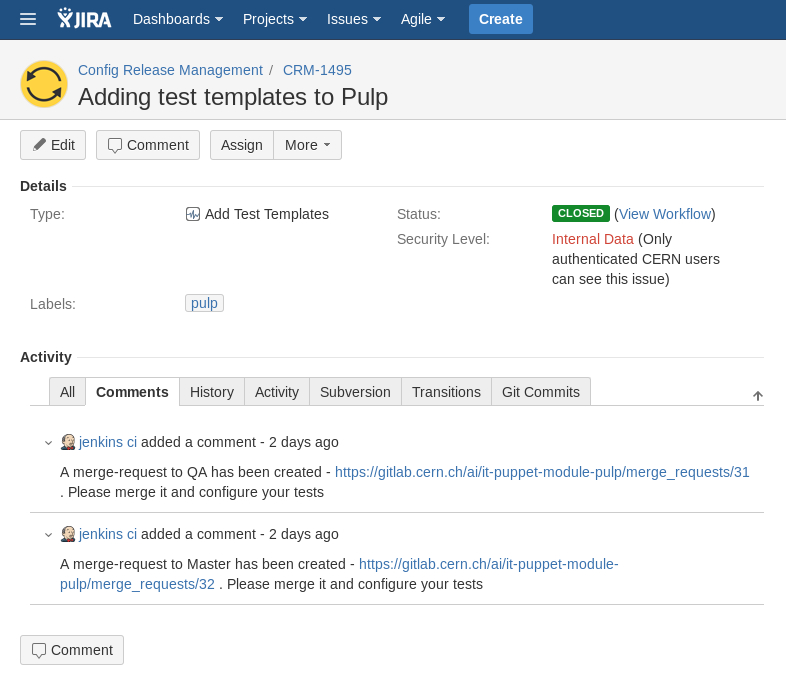
\includegraphics[width=\textwidth,height=\textheight,keepaspectratio]{ContinuousIntegrationWithJenkins/images/add_test_templates.jpg}
\end{figure}

This job scans Jira for tickets with type \textit{Add test templates} and
status \textit{Approved} and gets the module name from them. Then, it
clones the corresponding git repository of the module and, in a new branch
called \textit{add-tests} adds a folder containing all the test samples.
If all the operations are completed successfully, it creates two merge
requests on Gitlab: one from \textit{add-tests} to \textit{qa} and one to
\textit{master}. These requests need to be approved by the service manager
responsible for the module.

Following this, a new Jenkins jobs with the name of the module is created
(that will be triggered when a new CRM ticket is opened) and, if
everything goes well, the original Jira ticket is closed with status
\textit{Completed}. 

At this point the user can customize the tests and the Puppet manifests
that are present inside the module's repository merging the test samples
inside the repository and then editing them accordingly 

\subsubsection{Proposing a configuration change}

The procedure to propose a configuration change has not changed much but,
with added automation, users are less prone to make mistakes due to
repeating long procedures.

Once the user tested locally its module's change and wants to propose it
to the public all it has to do is: open a new ticket in Jira. Opening
a ticket requires multiple information that need to be provided by the
user: title, description, the module involved, the branch containing the
change and type equal to "Configuration Change". Since the use of the CI
is optional we added also a tick box to select if the user wants the
procedure to be handled by Jenkins or not.

\begin{figure}[H]
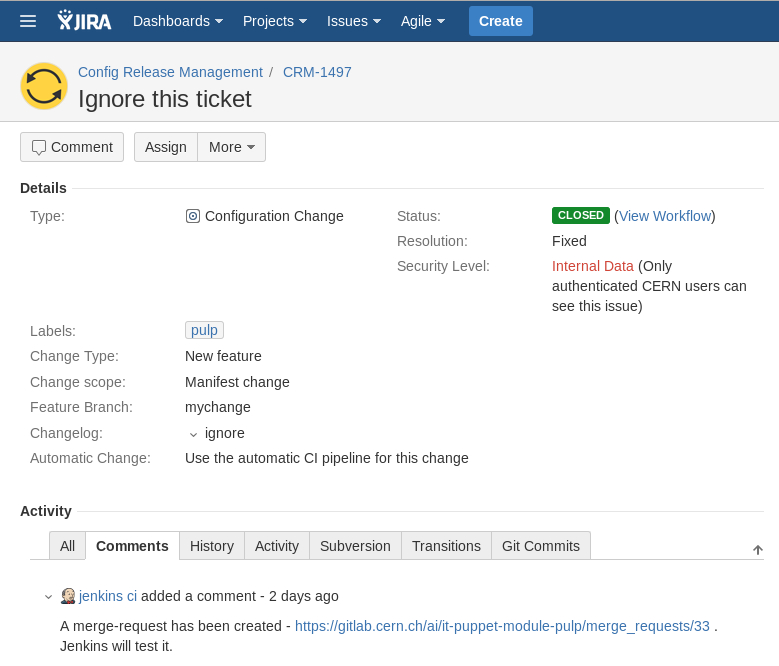
\includegraphics[width=\textwidth,height=\textheight,keepaspectratio]{ContinuousIntegrationWithJenkins/images/add_crm_change.jpg}
\end{figure}

When the user opens the ticket, the procedure is started, from now on the
whole work flow is automated and does not need any user interaction
(except, obviously, in case of tests failures).

Aidoctor, as described in the previous sections contains a script that
monitors the Jira service for new tickets. When the user creates a new
ticket this script forges a merge request on Gitlab using the ticket's
title and description, from the specified branch to the QA branch. The
link of the merge request is then posted in Jira to let the user have the
possibility to keep track of the work flow.

Jenkins monitors the Gitlab instance for new merge requests assigned to
the \textit{Jenkins CI} user, in fact we don't want our CI to take care of
all the merge requests. Whenever a new merge request is opened and the
assigner corresponds to the user associated with Jenkins a new build is
triggered. This means as well that users can test their changes using the
Continuous Integration infrastructure even without opening a CRM, but
simply assigning the merge request to Jenkins.

At this point Jenkins starts building the job called
\textit{it-puppet-module-modulename} with the parameters obtained from the
merge request. This job, that has been created in the previous sections
while adding the sample tests, consists in a set of sub-jobs:

\begin{enumerate}

  \item create-env

  Using as default QA. Overrides the module taken into consideration with
  the branch involved in the merge request.

  \item create-verify

  \item destroy-vm

  \item destroy-env

\end{enumerate}




